\documentclass[11pt]{article}
\usepackage[english]{babel}
\usepackage{bm}       % Required for bold math symbols
\usepackage{comment}
\usepackage{booktabs}
\usepackage{subcaption}
\usepackage{siunitx}
\usepackage{enumitem}
\usepackage[a4paper,top=2cm,bottom=2cm,left=2cm,right=2cm]{geometry}
\usepackage{amsmath}
\usepackage{graphicx}
\usepackage[colorlinks=true, allcolors=blue]{hyperref}
\captionsetup{font=footnotesize} % can also use \scriptsize
\usepackage{wrapfig}


% Adjust section title font sizes
\usepackage{titlesec}
%\titleformat*{\section}{\normalsize\bfseries}
%\titleformat*{\subsection}{\small\bfseries}
%\titleformat*{\subsubsection}{\small\bfseries}

\titlespacing*{\section}{0pt}{1ex}{0.5ex}
\titlespacing*{\subsection}{0pt}{1ex}{0.5ex}
\titlespacing*{\subsubsection}{0pt}{0.5ex}{0.5ex}

% Reduce space above and below figures
\setlength{\abovecaptionskip}{3pt}
\setlength{\belowcaptionskip}{0pt}
\setlength{\intextsep}{5pt} % Adjust this value as needed

\title{AS37: The Hubble diagram for type Ia supernovae}
\author{Candidate number: 1054940}

\begin{document}
\maketitle

%-------------------------------------------------------------------

\begin{abstract}
In this experiment we use a sample of 115 type Ia supernovae from the Supernova Legacy Survey to show that the universe is expanding. We try fitting different models, finding that a flat universe is consistent with the data. Even though the SNLS does not rule out non-flat models, independent microwave background measurements strongly suggest a flat universe. By combining the SNLS data with WMAP data we can also show that the universe expantion is accelerating (p value of $3.2 \times 10^{-5}$). 
\end{abstract}

%-------------------------------------------------------------------

\section{Introduction}
In this report we show how type Ia supernovae can be used as "standard candles", since we predict they explode at roughly the same mass, with the same brightness. This allows us to calculate the distance to the star. The speed of these stars relative to Earth is extracted from the red-shift of the light emitted caused by the Doppler Effect. The plot of the speed (or redness) versus time is called a Hubble diagram, after Edwin Hubble, who discovered that there is a linear dependence between the distance to a star and its velocity. 

The data we are analysing consists of the measured redshift and brightness value and its error for 115 supernovae from the "Supernovae Legacy Survey" \cite{SN_legacy_survey}. 


\section{Methods}
\subsection{Friedmann equation}
In this experiment we assume that the universe is uniform and isotropic \cite{AS37_lab_script}, which allows us to write the Friedmann equation: 
\begin{equation}
	H^2(a) = \left( \frac{\dot{a}}{a} \right)^2 = \frac{8 \pi G \rho}{3} - \frac{kc^2}{a^2} + \frac{\Lambda}{3}
	\label{eq:Friedmann}
\end{equation}
where $H(a)$ is the hubble parameter, $a$ is the scale factor, which is defined as 1 at the present time, $\rho$ is the density (due to matter and radiation), $k$ defines the geometry of the space ($k=0$ for a flat universe), and $\Lambda$ is the cosmological constant. We devide equation \eqref{eq:Friedmann} by $H^2$ to find the simplified relation: 
\begin{equation}
	1 = \Omega_M +\Omega_k + \Omega_\Lambda
	\label{eq:main}
\end{equation}
Note that we can use the Friedmann equation to thetermine if the universe's expantion is accelerating or decelerating. By multiplying equation \eqref{eq:Frierdmann} by $a^2$ and then differentiating we obtain: 
\begin{equation}
	2 \ddot{a} \dot{a} = -\frac{8 \pi G M}{3 a^2} \dot{a} + \frac{\Lambda 2 a}{3}  \dot{a}
\end{equation}
where we used $\rho = M/a^3$ for the denssity of matter. We can simplify and identify the terms from equation \eqref{eq:main}:
\begin{equation}
	\ddot{a} = -\frac{\Omega_M H^2}{2 a^2} + \Omega_{\Lambda} H^2 a
\end{equation}
For the present epoch, we have $a = 1$: 
\begin{equation}
	\ddot{a}_{\mathrm{present}} = H^2 \left(\Omega_{\Lambda,0} - \frac{\Omega_{M,0}}{2}\right)
	\label{eq:exp}
\end{equation}

\subsection{Flat universe}
It can be easily seen that if the universe is flat ($k = 0$), meaning that Euclidian geometry applies, or equivalently the angles of any triangle with the sides defined by light rays add up to $180^\circ$, then: 
\begin{equation}
	\Omega_M + \Omega_\Lambda = 1
	\label{eq:flat}
\end{equation}

\subsection{Dark energy}
The cosmological constant is a special case of a more general class of models called "dark energy" models. These models are characterised by the equation of state:
\begin{equation}
	P = w \rho c^2
	\label{eq:dark}
\end{equation}
which relates the pressure $P$ to the energy density $\rho c^2$. $w$ is a constant which is $w = -1$ for the special case of the Cosmological Constant. Also, the value $w = 0$ corresponds to normal matter. therefore we shouldn't try to fit $w = 0$ to the data since we are already accounting for normal matter with the $\Omega_M$ term. 

\subsection{The cosmological model}
There was another custom fitting model added to the qdp software: the "cosm" model which fits a Friedmann model to the data. This model has four parameters: the absolute magnitude to the Type 1a supernovae $AbsMag$, $\Omega_{M,0}$, $\Omega_{T,0} = \Omega_{M,0} + \Omega_{\Lambda,0}$ and the dark energy equation of state parameter $w$.

\section{Results}
\subsection{Linear fit}
We start with the simplest model, the one originally proposed by Edwin Hubble, which predicts a linear relation between the speed and distance of the observed stars. Since the apparent brightness of stars will decrease according to the inverse square law $S \propto d^{-2}$, we expect the slope of the linear fit to be $5$. This is because we are measuring brightness on the magnitude scale.
\begin{equation}
	m = -2.5\log_{10}\frac{S}{S_0}
	\label{eq:mag}
\end{equation}
where $m$ is the magnitude and  $S$ is the apparent brightness. Note that due to the minus sign, fainter objects have higher magnitudes. 

We fit the data with a linear $y = a + bx$ fit. We consider the parameter $a$ "uninteresting", meaning that we allow it to vary while fitting for $b$. We find the slope to be: 
\begin{equation}
	b = 5.50^{5.53}_{5.48} 
	\hspace{2cm}
	\chi^2 = 139.6
	\label{res:lin}
\end{equation}
The linear fit has a slope clearly different than $5$, which shows that this simple model does not adequately capture the physics at play. In figure \ref{fig:snls} we plot the dataset and the linear fit, together with the $b = 5$ linear fit. 
\begin{figure}[htbp]
	\centering
	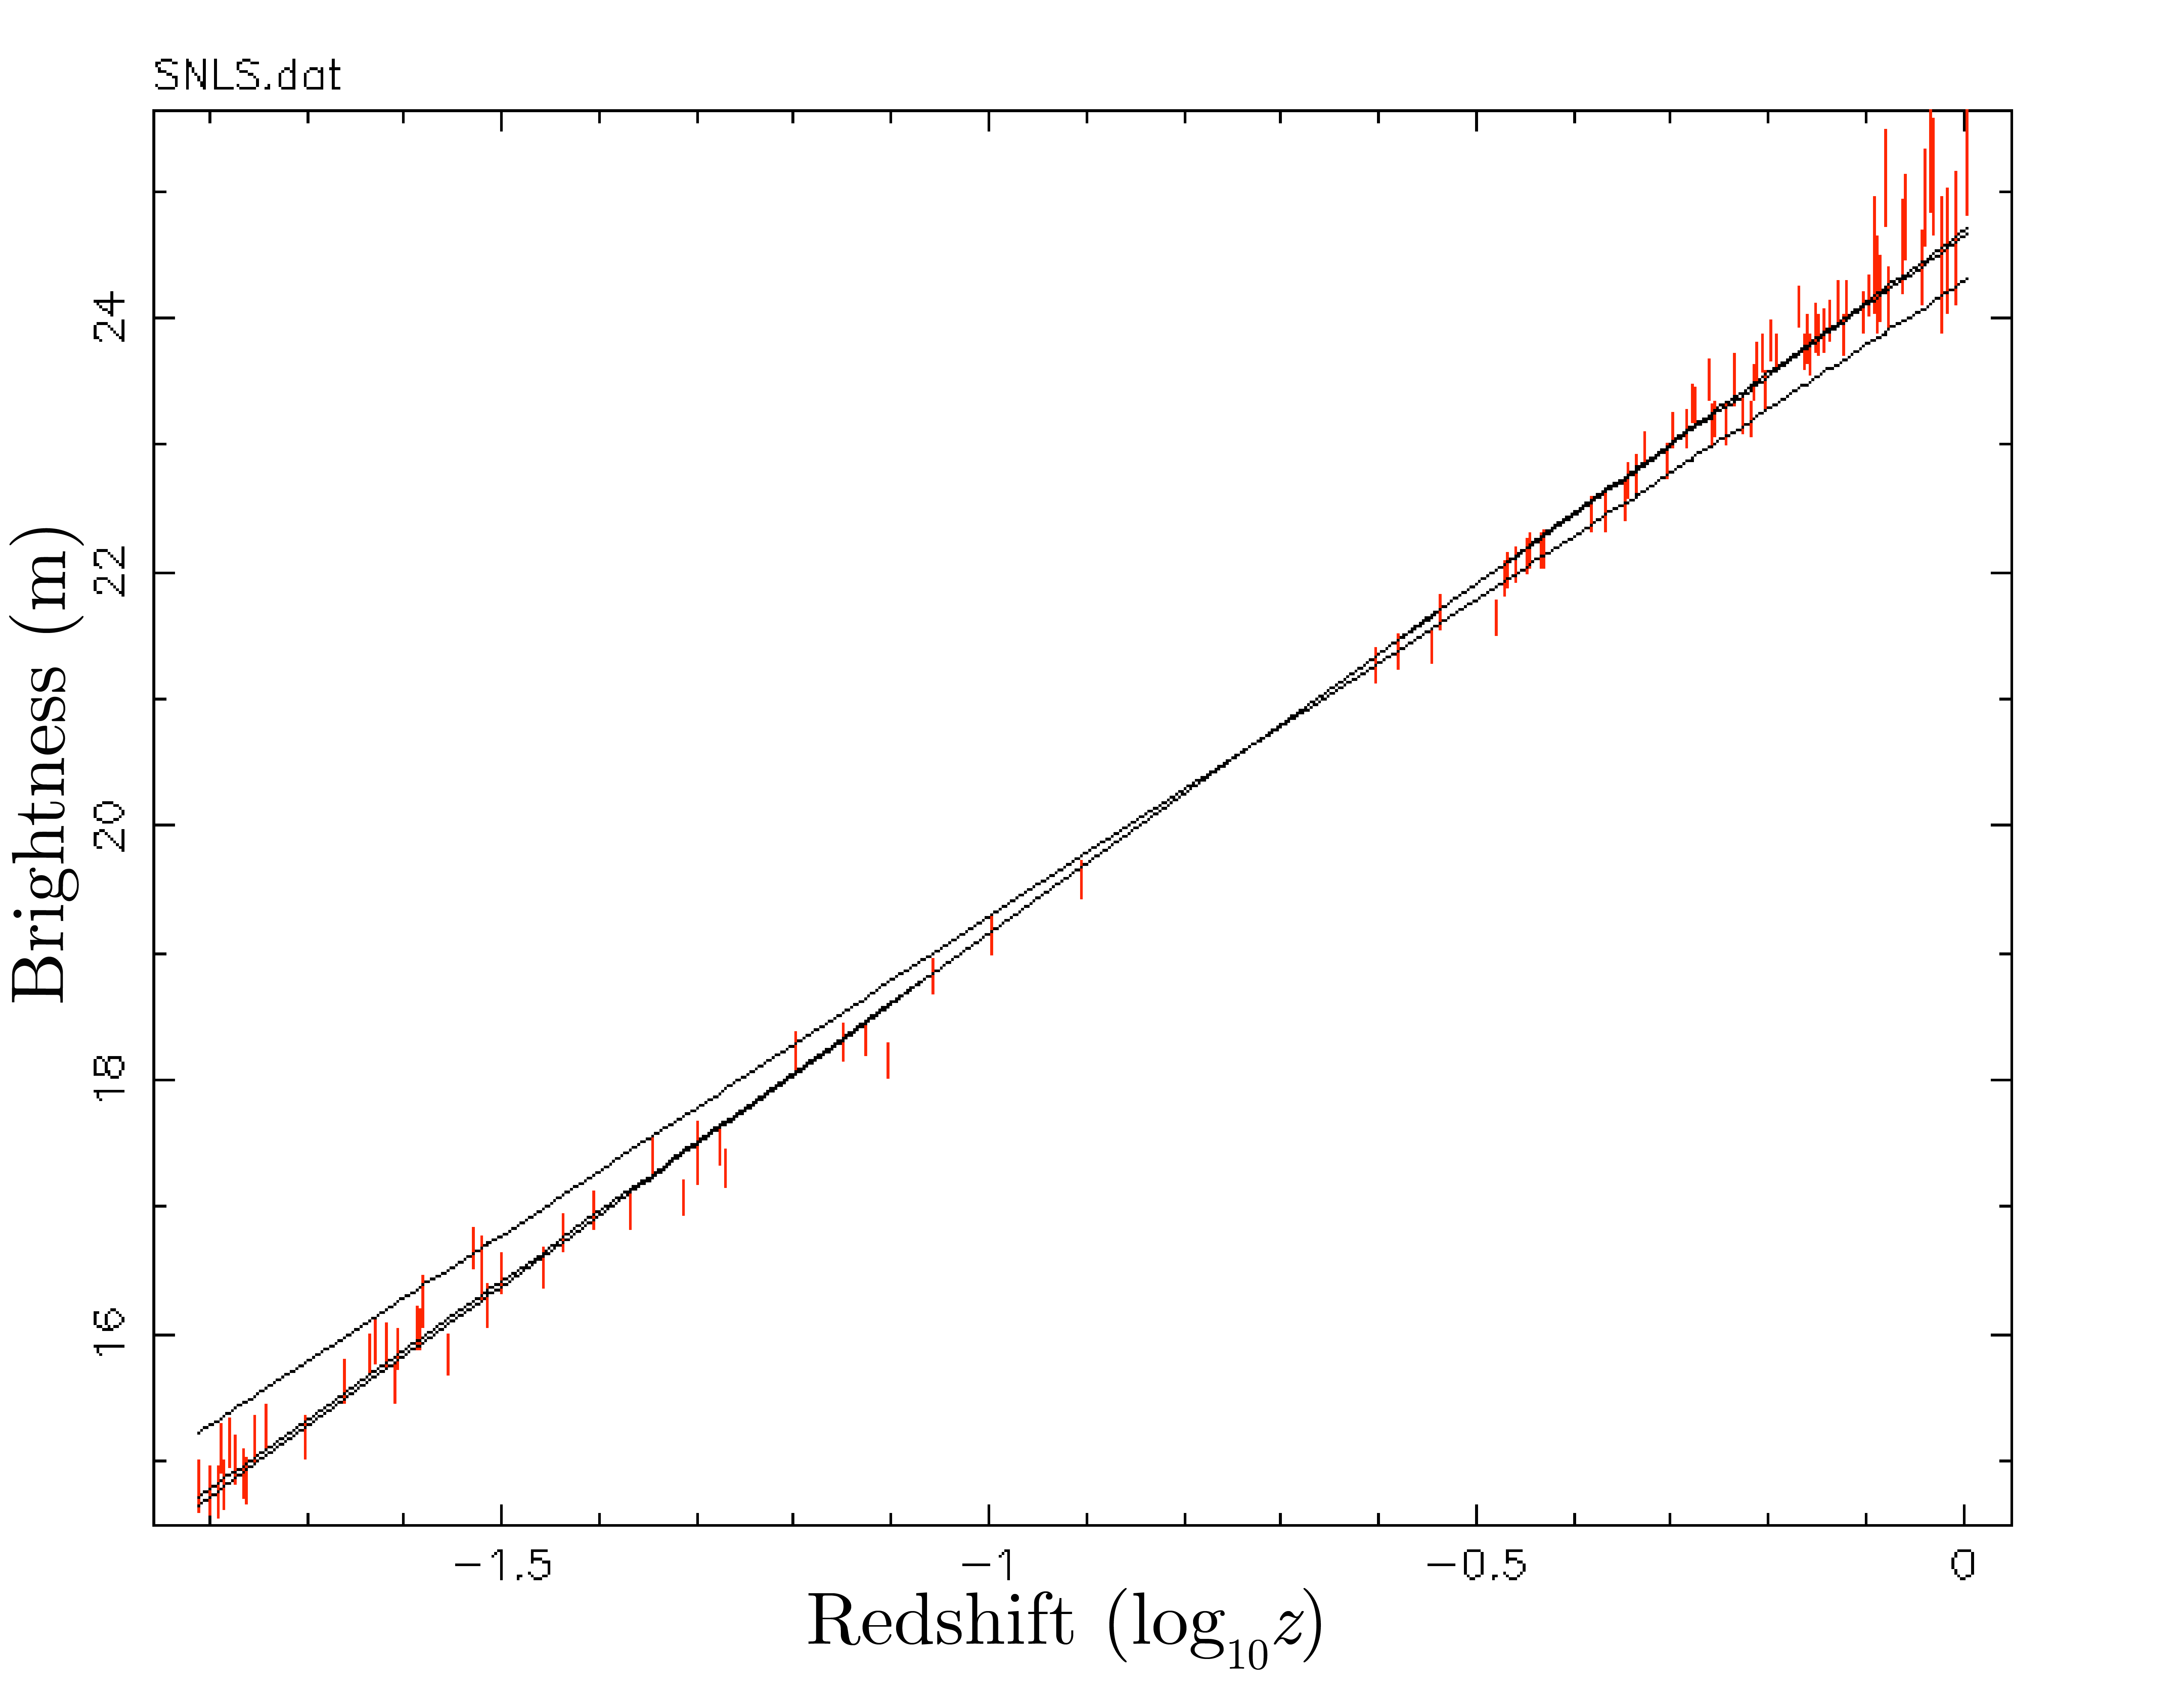
\includegraphics[width=0.8\linewidth]{snls.png}
	\caption{Type Ia supernovae data from the Supernovae Legacy Survey plotted on a Hubble diagram}
	\label{fig:snls}
\end{figure}
We also investigate if this simple model can be a good fit for a range of the data containing only the low redshift datapoints. Analysis of the $\chi^2$ value shows that the linear model breakes down after the first 43 data points, corresponding to a redshift of around $\log_{10}z = -0.95$. 

\subsection{Flat universe model} \label{sec:flat}
As stated before, we model a flat universe by setting $\Omega_{TOT,0} = \Omega_{M,0} + \Omega_{\Lambda,0} = 1$. We are also using the Cosmological Constant (set $w = -1$), which leaves  $\Omega_{M,0}$ and $AbsMag$ as the parameters to be fitted. We find: 
\begin{equation}
	\Omega_{M,0} = 0.26^{0.30}_{0.22} 
	\hspace{2cm}
	AbsMag = -19.247
	\hspace{2cm}
	\chi^2 = 110.9
	\label{res:flatM}
\end{equation}
Note that we did not investigate what is the $1\sigma$ confidence interval for the absolute magnitude of the SNe, since this is not the parameter we are interested in. Using equation \eqref{eq:flat} we find: 
\begin{equation}
	\Omega_{\Lambda,0} = 0.74^{0.88}_{0.70} 
	\label{res:flatL}
\end{equation}

MAYBE SAY THAT WE CHECKED THAT OMEGA INCREADES QUADRATICALLY
%If the uncertainties on the Hubble diagram are normally-distributed, the plot of χ2 v. parameter value should have a quadratic form. Try fitting a quadratic function to the plot using the standard model options in qdp (type mo to see the names of the model components that you can use, hint: you will need to use three components simultaneously to fit a quadratic function). Note that we don’t have uncertainties for the χ2 values themselves, so the goodness-of-fit returned by qdp in this case is meaningless - we just want a visual inspection to check things look sensible.



\subsection{Non-flat universe models}
We now turn to non-flat universe geometries ($\Omega_{TOT,0} $ is a free parameter), but still use the cosmological constant ($w = -1$). We find that we can not fit a single set of $\Omega_{M,0}$ and $\Omega_{\Lambda,0}$ to the data; there is a range of values that fit the data well (Figure \ref{fig:nonflat}). 
\begin{figure}[htbp]
	\centering
	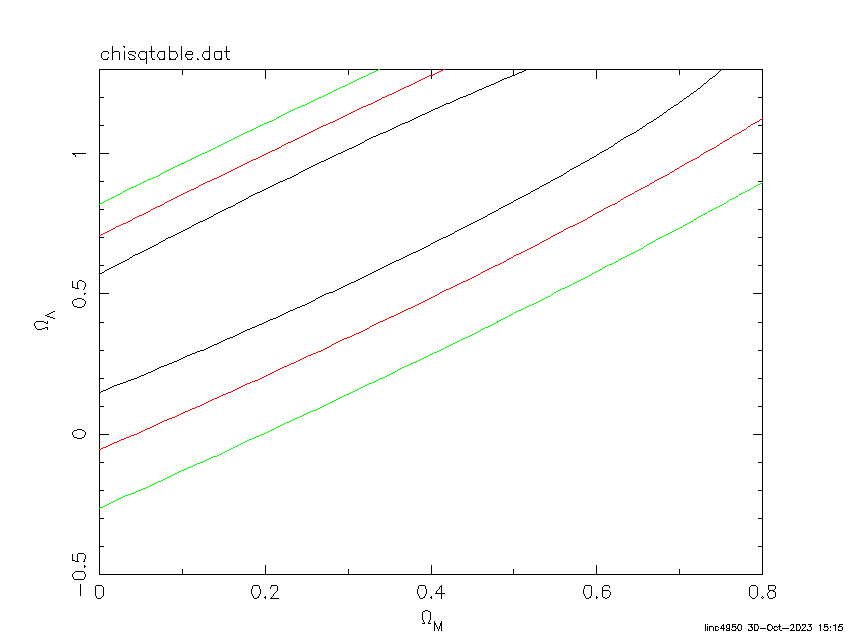
\includegraphics[width=0.8\linewidth]{nonflat.png}
	\caption{Contour plot of the 68\%, 90 \% and 99\% confidence intervals, plotted in black, red and green, respectively, for the cosmological parameters $\Omega_\Lambda$ and $\Omega_M$. The pair ($\Omega_\Lambda, \Omega_M$) can not be determined uniquely using only theSupernova Legacy Survey data.}
	\label{fig:nonflat}
\end{figure}

\subsection{Dark energy models}
When fitting for dark energy models there are two "interesting" parameters that we are manually fitting for: $\Omega_{M,0}$ and $w$. The four parameters are degenerate with each other, meaning that we can not fit all four parameters at the same time. 

Instead of assuming that the universe is perfectly flat, and directly fixing $\Omega_{TOT,0} = \Omega_{M,0} + \Omega_{\Lambda,0} = 1$, we can use the data from the microwave bacground observations, to further constrain the fit. The WMAP data predicts:
\begin{equation}
	\Omega_{k,0} = -0.014 \pm 0.017
	\label{res:WMAP}
\end{equation}
which is consistent with a flat universe, but still allows for some uncertainty. We obtain a very similar result (see Figure \ref{fig:dark}) to the one obtained in section \ref{sec:flat}, but the error bars are slightly bigger: 
\begin{equation}
	\Omega_{M,0} = 0.28 \pm 0.1
	\hspace{2cm}
	\Omega_{\Lambda,0} = 0.74 \pm 0.1
	\label{res:dark}
\end{equation}
\begin{figure}[htbp]
	\centering
	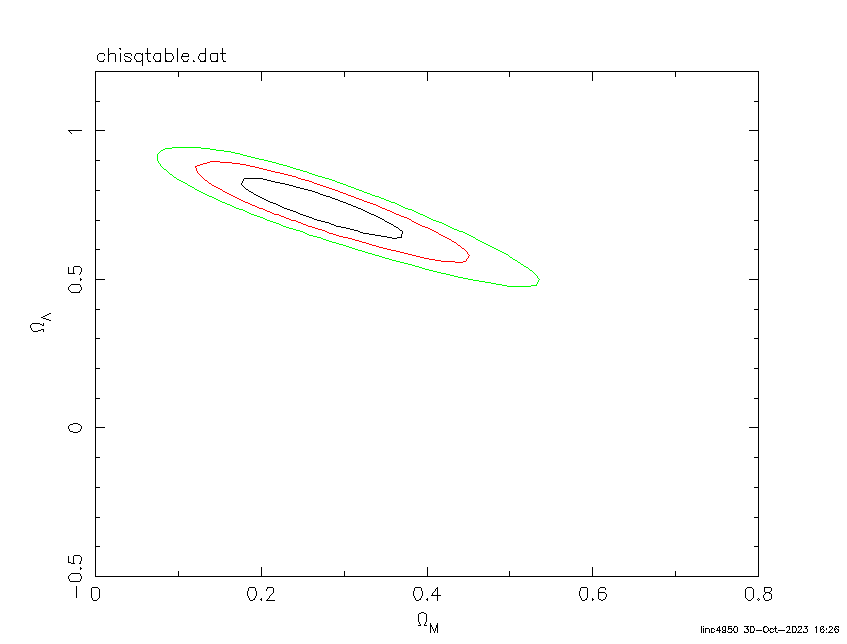
\includegraphics[width=0.8\linewidth]{dark.png}
	\caption{Contour plot of the 68\%, 90 \% and 99\% confidence intervals, plotted in black, red and green, respectively, for the cosmological parameters $\Omega_\Lambda$ and $\Omega_M$}
	\label{fig:dark}
\end{figure}
We use this data to find if the universe expansion is accelerating or decelerating by substituting the results \eqref{res:dark} into equation \eqref{eq:exp}. Note that the errors on the $\Omega_{M,0}$ and $\Omega_{\Lambda,0}$ results are highly corelated (Figure \ref{fig:dark}, therefore we can not reasonably just add the confidence intervals in quadrature. Instead we find that: 
\begin{equation}
	\Omega_{\Lambda,0} - \frac{\Omega_{M,0}}{2} = 0.60 \pm 0.15
\end{equation}
This means that the hypotesys that the universe's expansion is not accelerating is $4 \sigma$ away from measurements, allowing us to state that the universe's expansion is accelerating with a confidence of $1-p = 0.99997$. 

\section{Conclusions and further work}
In this experiment we showed how type Ia SNe can be used as "standard candles", allowing us to derive the distance to the supernovae. We can also use the redshift of the light coming from the SNe to determine their relative velocity to Earth. We showed that there is a range of cosmological parameters that fit this data well with a non-flat universe model. We also use an independent dataset of microwave background observations t determine that the universe is mostly flat. The combination of the two datasets allowa us to determine with $99.997\%$ confidence that the expansion of the universe is accelerating. 

Future work could focus on refining the measurements of cosmological parameters by incorporating more recent and comprehensive datasets of type Ia supernovae. Additionally, improving the calibration of supernova luminosities and reducing systematic uncertainties will enhance the precision of distance measurements. Expanding the analysis to include data from other cosmological probes, such as baryon acoustic oscillations (BAO) and gravitational lensing, could provide a more robust understanding of the universe's expansion history. Such independent measurements would be highly valuabe in verifying the validity of the models presented in this report. 

\bibliographystyle{plain}
\bibliography{bibliography}

%----------------------------------------------------------------
\newpage

\appendix
\section{some appendix} 
Some text

\end{document}